\chapter{Technische aspecten}
\section{Machine Learning}
\subsection{Inleiding}
\npar Leren is een veelzijdig fenomeen dat bestaat uit  verschillende processen: het verkrijgen van declaratieve kennis, het ontwikkelen van motorische en cognitieve vaardigheden door instructie en ervaring, het organiseren van nieuwe kennis in algemene representaties en het ontdekken van nieuwe feiten via observatie en experimentatie.
\npar Sinds het begin van het computertijdperk proberen onderzoekers het menselijk leren na te bootsen en deze processen te vertalen naar de informatietheorie. Het machinaal leren is nog steeds een erg uitdagend doel in de kunstmatige intelligentie (KI).

\npar Deze vorm van KI is dus volledig data gedreven tegenover traditionele methoden die zich beroepen op handgemaakte regels. Het computerprogramma wordt niet expliciet geprogrammeerd om een taak uit te voeren maar vertrekt vanuit een algemeen model. Het model leert eerst uit voorbeelden en kan daarna voorspellingen maken op nieuwe invoer.

\npar We kunnen zeggen dat een computerprogramma of machine leert als het zijn performantie op een bepaalde taak verbetert met ervaring \cite{machine_overview}.  Het leren gebeurt door de optimalisatie van de parameters van het predictief model door middel van een algoritme uit de machine learning. Het model wordt een aantal voorbeelden gegeven om uit te leren: de trainset. De uitvoer van het model wordt ge\"evalueerd aan de hand van een prestatiemaat. Deze prestatiemaat vertelt hoe correct de voorspelling is en bepaalt de mate waarin het model verder gecorrigeerd dient te worden.

\npar Machine learning algoritmes kunnen opgedeeld worden in drie categori\"en op basis van leerstijl: gesuperviseerd, ongesuperviseerd en semi-gesuperviseerd leren. De supervisie slaat op het gebruik van de correcte uitgangswaarde tijdens het trainen.

\npar Een ongesuperviseerde leerstijl vertrekt uit een dataset zonder klasselabels of correcte voorspellingswaarde. Er wordt een model opgebouwd die bepaalde structuren deduceert. Dit kan zijn om algemene regels te extraheren, om redundantie te verminderen of om gegevens te groeperen volgens gelijkenis (clustering).

\npar Bij gesuperviseerde methodes wordt een trainset gebruikt die zowel de invoervector als de te voorspellen waarde bevat. Problemen die vaak via gesuperviseerd leren worden aangepakt zijn classificatie en regressie. Classificatie tracht ingevoerde voorbeelden in te delen in discrete categori\"en om bijvoorbeeld objecten te herkennen zoals in \cite{krizhevsky2012imagenet}. Bij regressie is de uitvoer van het model een continue variabele zoals bijvoorbeeld de prijs van een appartement gegeven zijn oppervlakte.

\npar Semi-gesuperviseerde methodes zijn een mengvorm van de voorgaande twee. De dataset is een mengeling van gelabelde en ongelabelde voorbeelden. Hierbij is er een gewenste indeling, weergegeven door de gelabelde data, maar het model moet zelf de indeling zien te maken.


\subsection{Gesuperviseerde classificatie}

\npar De machine learning in dit onderzoek valt onder de gesuperviseerde classificatie. Een classificatieprobleem kan algemeen als volgt worden omschreven:
\npar Gegeven een trainset T:
\begin{equation}
T = \{ ( x^{(n)}, y^{(n)})\},\quad x^{(n)}\in\mathbb{R}^D, y^{(n)}\in\{0,1,...,C\}, n=1,...,N
\end{equation}
met $x^{(n)}$ het n-de datavoorbeeld en $y^{(n)}$ zijn klasselabel. C staat voor het aantal discrete categori\"en of klasses, D het aantal dimensies van de invoervariabelen en N het aantal trainingsvoorbeelden. Nu kunnen we het classificatieprobleem uitdrukken als de benadering van een model $f$ met parameters $\theta$:
\begin{equation}\label{eq:classifier}
f(x,\theta) = y,\quad\forall(x,y) \in T
\end{equation}
zodat we na deze schatting vanuit $f$ en $\theta$ voorspellingen kunnen maken op basis van nieuwe data: $f(x_{nieuw},\theta)=y', \quad y' \in\{0,1,...C\}$

\npar Figuur \ref{fig:alg-class-model} geeft een schematische weergave van de opbouw van een classificatiemodel. Het schatten van $f$ en $\theta$ wordt uitgevoerd door een techniek uit de machine learning en geeft ons het uiteindelijke predictief model $f(x,\theta) = y$. De samples worden meestal verwerkt voor ze als input worden doorgegeven aan het model. In het geval van classificatie van video en afbeeldingen worden er technieken uit de beeldverwerking gebruikt om relevante informatie uit het beeld te halen. Welke specifieke techniek er gebruikt wordt is een keuze die erg bewust moet gemaakt worden en een grote invloed heeft op de performantie van het classificatiemodel. Deze informatie wordt gebundeld in een featurevector ($x$) en aan het ML algoritme gegeven. Vanuit de verkregen featurevectoren en de kennis van het correcte klasselabel wordt het predictief model dan geoptimaliseerd.
\npar Eenmaal het model voldoende geleerd heeft kan het predictief model gebruikt worden in een productieomgeving om nieuwe voorbeelden, al dan niet correct, te classificeren.
\npar Het model dat in dit onderzoek gebruikt wordt is dat van het artificieel neuraal netwerk, een veel gebruikt predictief model voor classificatie. In sectie \ref{sec:ann} wordt deze techniek dan ook verder besproken.
\begin{figure}
	\centering
	\def\svgscale{0.85}
%	\def\svgwidth{\columnwidth}
	\input{figuren/figuur-classificatieML.pdf_tex}
	\caption{Schematische weergave van het opstellen van een predictief model met behulp van machine learning technieken \label{fig:alg-class-model}}
\end{figure}

\subsection{Overfitting}
\npar Stel dat je naar een symfonisch orkest gaat luisteren in een schouwburg en je wilt het meest klare en pure geluid mogelijk ervaren. Je koopt een hooggevoelige microfoon en hoorapparaat en probeert zo alle geluiden op te nemen in het auditorium. Nu hoor je naast het geluid van het symfonisch orkest ook alle ruis. Je hoort de mensen schuiven in hun stoelen, de muzikanten die hun muziekpapier omslaan en het gezwiep van de dirigent zijn baton. Dit fenomeen wordt overfitting genoemd. Als je op een concert bent is er zowel de symfonie als de willekeurige ruis. Een perfect en algemeen model luistert enkel naar de symfonie. Overfitting is wanneer je meer ruis hoort dan noodzakelijk, of erger, als je de ruis boven de symfonie hoort.

\npar Bij overfitting beschrijft het predictief model de ruis en fouten in het signaal in plaats van de gewenste onderliggende patronen en kenmerken van de gegeven taak. Het komt voor wanneer het model complex is en vele parameters heeft in vergelijking met het aantal trainingsvoorbeelden. Een model dat ``overfit'' is heeft een laag voorspellend vermogen op ongeziene data. Het model is niet algemeen of gegeneraliseerd en  \textit{memoriseert} de data. 

\begin{figure}
	\centering
	\def\svgscale{0.7}
	%	\def\svgwidth{\columnwidth}
	\input{figuren/overfitting.pdf_tex}
	\caption{Plot van trainings- en validatiefout ter illustratie van overfitting en de early stopping techniek.}
	\label{fig:overfitting}
\end{figure}

\npar Het risico op overfitten komt uit het feit dat de prestatiemaat voor de training van het model niet correct de effectiviteit van het model weergeeft. De training van een model gebeurt doorgaans via optimalisatie van zijn prestatie op een training set. De werkelijke performantie wordt echter gegeven door prestatie op ongeziene data. Net om deze reden wordt de dataset opgesplitst in drie delen: training-, validatie- en testset.
\npar Om een zo goed mogelijk predictief model te maken wordt een evaluatiescore op de validatieset geminimaliseerd of gemaximaliseerd. Deze data is nog onbekend voor het model en geeft dus een betere aanduiding van zijn performantie. Figuur \ref{fig:overfitting} geeft de validatie- en trainingsfout weer tijdens het trainen van een predictief model. Wanneer de trainingsfout blijft dalen maar de validatiefout stagneert of stijgt is er sprake van overfitting. Nu kan er gekozen worden om de training vroegtijdig te stoppen teneinde geen generalisatie te verliezen. Deze techniek wordt \textit{early stopping} genoemd.

\npar Om na afloop een finale evaluatie van het model te maken wordt zijn prestatie op de testset gemeten. De testset mag nooit gebruikt worden om aanpassingen aan het model te maken maar dient enkel voor een eindevaluatie.







\section{Artificieel neuraal netwerk}\label{sec:ann}
\subsection{Inleiding}
\begin{figure}
	\centering
	\begin{subfigure}{.5\textwidth}
		\centering
		\input{figuren/neuron.pdf_tex}
		\caption{Artificieel neuron.}
		\label{fig:neuron}
	\end{subfigure}%
	\begin{subfigure}{.5\textwidth}
		\centering
		\input{figuren/ANN-alg.pdf_tex}
		\caption{Artificieel neuraal netwerk}
		\label{fig:ANN}
	\end{subfigure}
	\caption{Een ANN met een invoerlaag, twee verborgen lagen en een softmax uitvoerlaag samen met zijn bouwsteen, het artificieel neuron.}
	\label{fig:test}
\end{figure}
Een lange rekensom uitwerken is iets wat de mens liever overlaat aan een rekenmachine of computer. Alle bits van een rekensom zijn even belangrijk en bepalend voor zijn uitkomst. Op dit vlak is een computer veel effici\"enter en betrouwbaarder dan ons brein. Onze hersenen zijn veel bedrevener in andere taken zoals het indelen van objecten volgens gelijkenis of het herkennen van een persoon.
\npar Het is deze gedachte die vele onderzoekers ertoe bracht een artificieel neuraal netwerk (ANN) uit te bouwen. Het menselijke brein is een erg complex neuraal netwerk bestaande uit meer dan 86 miljard neuronen. Dit zijn de bouwstenen van ons zenuwstelsel en ze staan in voor het verwerken en overdragen van informatie. In figuur \ref{fig:neuron} is een weergave te zien van een artificieel neuron, de bouwsteen van het ANN. De functionaliteit van dit neuron bootst deze van het biologisch neuron na en wordt als volgt gedefini\"eerd:
\begin{equation}\label{eq:neuron}
n = a\bigg(b+\sum_{i=1}^{D}w_ix_i\bigg)
\end{equation}
met $n$ de uitvoer van het neuron, $a$ de \textit{activatiefunctie}, $b$ de bias, $x_i$ de $i$-de invoer en $w_i$ de gewichten van zijn respectievelijke inkomende verbindingen.



\npar Deze artifici\"ele neuronen worden gegroepeerd in lagen om een ANN te vormen zoals afgebeeld in figuur \ref{fig:ANN}. Alle lagen worden onderling volledig verbonden, elk neuron krijgt invoer van alle neuronen uit de voorgaande laag en geeft zijn uitvoer door aan alle neuronen van de volgende laag. Deze lagen worden dan ook vaak \textit{dense layers} genoemd vanwege hun verbindingsdichtheid.
\npar Hier beschouwen we enkel \textit{feedforward neurale netwerken}. Aan het begin van het netwerk hebben we de invoerlaag met evenveel knopen als de dimensie van de featurevectoren. De invoer propageert zich van links naar rechts door het netwerk tot het bij de uitvoerlaag komt. Omdat de uitvoer van de binnenste lagen niet meteen zichtbaar is worden deze de verborgen lagen genoemd.
\npar De uitvoer van de verschillende lagen uit het ANN in figuur \ref{fig:ANN} kunnen we als volgt beschrijven:
\begin{equation}
\begin{aligned}
h^{(1)}_j\quad=&\quad a\bigg(\sum_{i=1}^{D}w^{(1)}_{i,j}x_i\bigg),\quad j=1,...,M_1\\
h^{(2)}_j\quad=&\quad a\bigg(\sum_{i=1}^{M_1}w^{(2)}_{i,j}h^{(1)}_i\bigg),\quad j=1,...,M_2\\ 
y_j\quad=&\quad a\bigg(\sum_{i=1}^{M_2}w^{(3)}_{i,j}h^{(2)}_i\bigg),\quad j=1,...,C 
\end{aligned}
\end{equation}
met $D$ het aantal invoerparameters, $M_1$ het aantal verborgen knopen in de eerste laag, $M_2$ het aantal verborgen knopen in de tweede laag en $C$ het aantal te voorspellen klassen. $M_1$ en $M_2$ zijn hyperparameters van het model die geoptimaliseerd worden door de evaluatie van het model tegenover de validatieset.
\npar Het is mogelijk en wenselijk om nog meer verborgen lagen toe te voegen. Het omkaderde gedeelte in figuur \ref{fig:ANN} kan een aantal keer herhaald worden om zo het model toe te laten een complexere structuur te modelleren.
\begin{figure}[ht]
	\begin{center}
		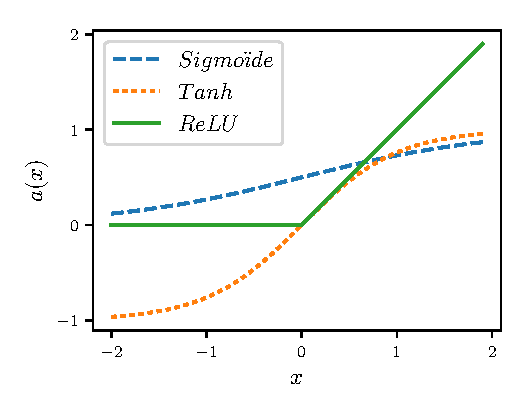
\includegraphics[width=8cm,keepaspectratio]{figuren/activatiefuncties.pdf}
		\caption{Weergave van de drie meest populaire activatiefuncties voor classificatie doeleinden \label{fig:activatie-fun}}
	\end{center}
\end{figure}
\npar De activatiefunctie $a(x)$ uit (\ref{eq:neuron}) is van groot belang in een ANN aangezien ze zorgt voor een niet-lineariteit. Moest deze er niet zijn kan elk neuraal netwerk met een verborgen laag vervangen worden door een model zonder aangezien de samenstelling van lineaire transformaties zelf een lineaire transformatie is. Figuur \ref{fig:activatie-fun} geeft drie van de meeste gebruikte niet lineaire activatiefuncties weer. In dit onderzoek zal gebruik gemaakt worden van de rectifier activatiefunctie:
\begin{equation}
\quad a(x) = max(0,x)
\end{equation}
Een neuron wordt vaak vernoemd naar de activatiefunctie die ze gebruikt. In dit geval spreken we van een Rectified Linear Unit (ReLU). Het gebruik van ReLU's wordt gestaafd door vele onderzoekswerken omtrent gesuperviseerde \textit{deep learning} zoals \cite{ReLU} en \cite{lionel}. Een ReLU zal alle negatieve waarden afbeelden op 0 en alle positieve op zichzelf.

\subsection{Leren}
%What has attracted the most interest in neural networks is the possibility of learning. Given a specific task to solve, and a class of functions F {\displaystyle \textstyle F} \textstyle F, learning means using a set of observations to find f ∗ ∈ F {\displaystyle \textstyle f^{*}\in F} \textstyle f^{*}\in F which solves the task in some optimal sense.
%
%This entails defining a cost function C : F → R {\displaystyle \textstyle C:F\rightarrow \mathbb {R} } \textstyle C:F\rightarrow \mathbb {R} such that, for the optimal solution f ∗ {\displaystyle \textstyle f^{*}} \textstyle f^{*}, C ( f ∗ ) ≤ C ( f ) {\displaystyle \textstyle C(f^{*})\leq C(f)} \textstyle C(f^{*})\leq C(f) ∀ f ∈ F {\displaystyle \textstyle \forall f\in F} \textstyle \forall f\in F – i.e., no solution has a cost less than the cost of the optimal solution (see mathematical optimization).
%
%The cost function C {\displaystyle \textstyle C} \textstyle C is an important concept in learning, as it is a measure of how far away a particular solution is from an optimal solution to the problem to be solved. Learning algorithms search through the solution space to find a function that has the smallest possible cost.
%
%For applications where the solution is dependent on some data, the cost must necessarily be a function of the observations, otherwise we would not be modelling anything related to the data. It is frequently defined as a statistic to which only approximations can be made. As a simple example, consider the problem of finding the model f {\displaystyle \textstyle f} \textstyle f, which minimizes C = E [ ( f ( x ) − y ) 2 ] {\displaystyle \textstyle C=E\left[(f(x)-y)^{2}\right]} \textstyle C=E\left[(f(x)-y)^{2}\right], for data pairs ( x , y ) {\displaystyle \textstyle (x,y)} \textstyle (x,y) drawn from some distribution D {\displaystyle \textstyle {\mathcal {D}}} \textstyle {\mathcal {D}}. In practical situations we would only have N {\displaystyle \textstyle N} \textstyle N samples from D {\displaystyle \textstyle {\mathcal {D}}} \textstyle {\mathcal {D}} and thus, for the above example, we would only minimize C ^ = 1 N ∑ i = 1 N ( f ( x i ) − y i ) 2 {\displaystyle \textstyle {\hat {C}}={\frac {1}{N}}\sum _{i=1}^{N}(f(x_{i})-y_{i})^{2}} \textstyle {\hat {C}}={\frac {1}{N}}\sum _{i=1}^{N}(f(x_{i})-y_{i})^{2}. Thus, the cost is minimized over a sample of the data rather than the entire distribution generating the data.
%
%When N → ∞ {\displaystyle \textstyle N\rightarrow \infty } \textstyle N\rightarrow \infty some form of online machine learning must be used, where the cost is partially minimized as each new example is seen. While online machine learning is often used when D {\displaystyle \textstyle {\mathcal {D}}} \textstyle {\mathcal {D}} is fixed, it is most useful in the case where the distribution changes slowly over time. In neural network methods, some form of online machine learning is frequently used for finite datasets.
%\subsection{Gradient descent}

\section{Convolutioneel neuraal netwerk}
De vloek van de dimensionaliteit: 
\subsection{Tweedimensionale convolutie}
\subsection{Maximum pooling}
\begin{figure}
	\centering
%	\def\svgscale{0.85}
	%	\def\svgwidth{\columnwidth}
	\input{figuren/max-pooling.pdf_tex}
	\caption{Maximum pooling: uit elk vak in de invoer afbeelding wordt het maximum bepaald en overgenomen in de bijhorende pixel in het uitvoerbeeld.}
	\label{max-poolingl}
\end{figure}

\section{Hyperparameters}
\subsection{Momentum}
\subsection{Dropout}\label{sec:dropout}


\cite{dropout}
\subsection{Data-augmentatie}\label{sec:data-augm}